\documentclass[11pt, a4paper]{article}

\usepackage[utf8]{inputenc}
\usepackage[T1]{fontenc}

\usepackage{amsmath,amssymb,amsthm,amsfonts,graphicx,float,fullpage,booktabs, bm} 
\usepackage[colorlinks,citecolor=blue,bookmarks=true]{hyperref}
\hypersetup{linkcolor=blue}
\usepackage{cleveref}
% Code listings
\usepackage{minted}
\usepackage{caption}
\usemintedstyle[python]{manni}
\usemintedstyle[R]{manni}

\usepackage{todonotes}

\title{\vspace{-8ex} \huge \bfseries Stochastic Processes\\
	\LARGE \normalfont \textsc{Assignment One} \vspace{-2ex}}
\author{\bfseries Santiago Alfonso Raposo Briceño - 100414456 \\
		\bfseries Javier Martínez Llamas - 100392684\\
		\bfseries Ricardo Hortelano Sánchez - 100418220}
\date{\vspace{-5ex}} % Remove space where date would be.

\begin{document}
\maketitle
\hrule

\section{Problem 1}

\subsection{Question a}
We can model the different channels as states in a Markov chain, with two absorbing states representing the conversion or non-conversion of a client.
This assumes however that the channel each user explores is only decided by the last channel he or she clicked on, which might not be completely realistic.

\subsection{Question b}
The state space is all of the unique values of the chain existing in our sample. This is easily computed with R, and it appears our state space consists of:
\begin{itemize}
	\item \textbf{Three channels} labeled as \verb|Ch 1|, \verb|Ch 2| and \verb|Ch 3|.
	\item \textbf{Two absorbing states} representing the \verb|Conversion| and \verb|Non-conversion| states.
\end{itemize}

We found the estimate of the transition probabilities using maximum likelihood, as we have from our notes:
\[
	\hat p_{ij} = \frac{n_{ij}}{\sum_{j = 1}^{k}} j,i \in S
\]
Where $n_{ij}$ is the total number of transitions from state $i$ to state $j$ and the denominator is the total amount of transitions \emph{into} state $j$.
The estimate found for our sample is the following transition matrix:
\[
 P = \begin{bmatrix}
 	0.3042 & 0.0792 & 0.1518 & 0.3132 & 0.1515 \\
 	0.1660 & 0.1612 & 0.3365 & 0.1601 & 0.1761 \\
 	0.1358 & 0.0756 & 0.1459 & 0.2202 & 0.4225 \\
 	0.0000 & 0.0000 & 0.0000 & 1.0000 & 0.0000 \\
 	0.0000 & 0.0000 & 0.0000 & 0.0000 & 1.0000
 \end{bmatrix},
\]
where we have encoded our states as numbers using the following mapping: \verb|Ch 1| is row (and column) 1, \verb|Ch 2| is number 2, \verb|Ch 3| is number 3, \verb|Conversion| is number 4 and \verb|Non-Conversion| is number 5.

\subsection{Question c}
Our first consumer journey is \verb|Ch 3 -> Ch 2 -> Conversion|, which is equivalent in our numerical mapping to $X_1 = 3, X2 = 2, X3 = 4$.
The probability we then have to calculate is $P(X_3 = 4|X_2=2, X_1 = 3)$. This can be done as follows:
\begin{align*}
	&P(X_3 = 4|X_2=2, X_1 = 3) = P(X_3 = 4 | X_2 = 2) * P(X_2 = 2 | X_1 = 3) * P(X_1 = 3) \\
	&= P_{2,4} * P_{3,2} * (\bm{\alpha}P)_3
\end{align*}
Assuming our initial distribution $\bm{\alpha} = (\frac{1}{3}, \frac{1}{3}, \frac{1}{3}, 0, 0)$\footnote{We are assuming the client cannot start in one of the conversion or non-conversion states and that it is uniform on the rest, which seems reasonable.} the answer is $0.0026$.

\subsection{Question d}
We can find the limiting distribution for the chain by using the result from equation 3.11 in Dobrow. This allows us to compute the limiting submatrix as $ \bm{(I-Q)^{-1}R}$ for the absorbing states, which is:
\[
	\bm{(I-Q)^{-1}R} = \begin{bmatrix}
		0.5887 & 0.4113 \\
		0.4650 & 0.5350 \\
		0.3925 & 0.6075
	\end{bmatrix}
\]
Where the first column represents the limiting distribution of the conversion state and the second column represents the limiting distribution of the non-conversion state. 
We can then compute the total conversion ratio as the ratio between the sum of column 1 (which is the total proportion of realizations that end in a conversion) divided by the sum of the matrix.
\[
	\text{Conversion Ratio }  = 0.4821.
\]

\subsection{Question e}
We get the following results for the two approaches to calculating the removal effect.
\begin{table}[H]
	\centering  
	\begin{tabular}{clccc}
		\toprule
		          Approach            & State & Removal Effect &  &  \\ \midrule
		Completely removing the state & Ch 1  &     0.2085     &  &  \\
		                              & Ch 2  &    -0.0285     &  &  \\
		                              & Ch 3  &    -0.2328     &  &  \\ 
		Making the state ``useless''  & Ch 1  &     0.5921     &  &  \\
		                              & Ch 2  &     0.4013     &  &  \\
		                              & Ch 3  &     0.4681     &  &  \\ \bottomrule
	\end{tabular}
	\caption{Removal effect of both approaches}
	\label{tab:removal-effect}
\end{table}
The conversion ratio is defined as $1 - \frac{CR_{new}}{CR_{old}}$. We can see then that if the new conversion ratio is smaller than the old conversion ratio, the removal effect will be positive and it will be negative otherwise.
Seeing \cref{tab:removal-effect} we can conclude that:
\begin{itemize}
	\item \textbf{Channel 1} always has a positive removal effect, which means that removing it causes the new conversion rate to be lower than the global conversion rate. Both approaches then seem to indicate that removing channel one would be counterproductive, as it is contributing to a high amount of conversions.
	\item \textbf{Channel 2} does not seem to change the conversion rate much with the first approach, but for the second approach it does make the new conversion rate lower. Therefore we can assume that this state is maybe not as important as the first one, but it does have a positive impact on the conversion rate.
	\item The removal of \textbf{Channel 3} actually has contradicting results for the two strategies. In the first one, removing it actually raises the conversion rate, but with the second approach its removal decreases the conversion rate by almost half. We would have to further examine why this is the case to conclude whether the removal of this channel would affect the conversion rate positively or not.
\end{itemize}

\section{Question 2}
\subsection{Question a}
We can see the transition graph in \cref{fig:trans-graph}.
\begin{figure}[H]
	\centering
	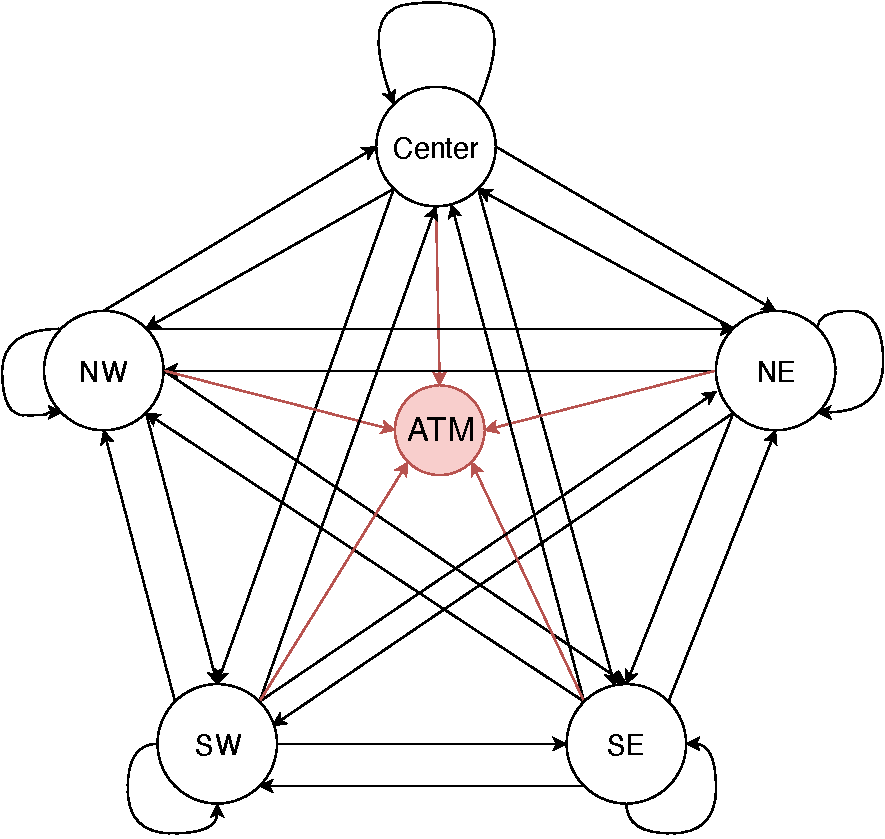
\includegraphics[scale = .7]{figures/transition-graph.pdf}
	\caption{Transition Graph}
	\label{fig:trans-graph}
\end{figure}
The state \verb|Atm| represents a particle escaping into the atmosphere, and it is the only absorbing state. The other states are all transient and aperiodic (as they all have loops to themselves).

We have not represented the probabilities in the graph as they are not given and it would be quite noisy. The arrows indicate that in principle the states are all connected with each other (in both directions).
\end{document}
